\documentclass[11pt,professionalfonts,hyperref={pdftex,pdfpagemode=none,pdfstartview=FitH}]{beamer}
%\usepackage{times}
%\usefonttheme{serif}
%\usepackage{helvet}
%\usepackage{amsmath,amssymb}
\usepackage{graphicx,multirow}

%\usepackage{movie15}
\usepackage{media9}

\usepackage{caption}
\usepackage{subcaption}
\captionsetup{compatibility=false}


%\usepackage{warmread}
%\usepackage[all,import]{xy}

%\renewcommand\mathfamilydefault{\rmdefault}

% JIRS includes
%\usepackage{graphicx}
%\usepackage{amsmath,amssymb,url,times}%,subfigure}% amsthm is the one!
%\usepackage{caption,subcaption,hyperref}
%\usepackage{color,comment}
%\usepackage{curves,pgfgantt}

\newcommand{\norm}[1]{\ensuremath{\left\| #1 \right\|}}
\newcommand{\bracket}[1]{\ensuremath{\left[ #1 \right]}}
\newcommand{\braces}[1]{\ensuremath{\left\{ #1 \right\}}}
\newcommand{\parenth}[1]{\ensuremath{\left( #1 \right)}}
\newcommand{\pair}[1]{\ensuremath{\langle #1 \rangle}}
\newcommand{\met}[1]{\ensuremath{\langle\langle #1 \rangle\rangle}}
\newcommand{\refeqn}[1]{(\ref{eqn:#1})}
\newcommand{\reffig}[1]{Fig. \ref{fig:#1}}
\newcommand{\tr}[1]{\mathrm{tr}\ensuremath{\negthickspace\bracket{#1}}}
\newcommand{\trs}[1]{\mathrm{tr}\ensuremath{[#1]}}
\newcommand{\deriv}[2]{\ensuremath{\frac{\partial #1}{\partial #2}}}
\newcommand{\SO}{\ensuremath{\mathsf{SO(3)}}}
\newcommand{\T}{\ensuremath{\mathsf{T}}}
\renewcommand{\L}{\ensuremath{\mathsf{L}}}
\newcommand{\so}{\ensuremath{\mathfrak{so}(3)}}
\newcommand{\SE}{\ensuremath{\mathsf{SE(3)}}}
\newcommand{\se}{\ensuremath{\mathfrak{se}(3)}}
\renewcommand{\Re}{\ensuremath{\mathbb{R}}}
\newcommand{\aSE}[2]{\ensuremath{\begin{bmatrix}#1&#2\\0&1\end{bmatrix}}}
\newcommand{\ase}[2]{\ensuremath{\begin{bmatrix}#1&#2\\0&0\end{bmatrix}}}
\newcommand{\D}{\ensuremath{\mathbf{D}}}
\newcommand{\Sph}{\ensuremath{\mathsf{S}}}
\renewcommand{\S}{\Sph}
\newcommand{\J}{\ensuremath{\mathbf{J}}}
\newcommand{\Ad}{\ensuremath{\mathrm{Ad}}}
\newcommand{\intp}{\ensuremath{\mathbf{i}}}
\newcommand{\extd}{\ensuremath{\mathbf{d}}}
\newcommand{\hor}{\ensuremath{\mathrm{hor}}}
\newcommand{\ver}{\ensuremath{\mathrm{ver}}}
\newcommand{\dyn}{\ensuremath{\mathrm{dyn}}}
\newcommand{\geo}{\ensuremath{\mathrm{geo}}}
\newcommand{\Q}{\ensuremath{\mathsf{Q}}}
\newcommand{\G}{\ensuremath{\mathsf{G}}}
\newcommand{\g}{\ensuremath{\mathfrak{g}}}
\newcommand{\Hess}{\ensuremath{\mathrm{Hess}}}
\newcommand{\refprop}[1]{Proposition \ref{prop:#1}}
\newcommand{\argmax}{\operatornamewithlimits{argmax}}

\definecolor{mygray}{gray}{0.9}

\graphicspath{{../../Fig/}}

\mode<presentation> {
  \usetheme{Warsaw}
  \usefonttheme{serif}
  \setbeamercovered{transparent}
}

\newcommand{\mypaper}{}

\setbeamertemplate{footline}%{split theme}
{%
  \leavevmode%
  \hbox{\begin{beamercolorbox}[wd=.85\paperwidth,ht=2.5ex,dp=1.125ex,leftskip=.3cm,rightskip=.3cm plus1fill]{author in head/foot}%
    \usebeamerfont{author in head/foot}\insertshorttitle
  \end{beamercolorbox}%
  \begin{beamercolorbox}[wd=.15\paperwidth,ht=2.5ex,dp=1.125ex,leftskip=.3cm,rightskip=.3cm]{title in head/foot}
    \usebeamerfont{title in head/foot}\mypaper\hfill \insertframenumber/\inserttotalframenumber
  \end{beamercolorbox}}%
  \vskip0pt%
} \setbeamercolor{box}{fg=black,bg=yellow}

\title[Autonomous Aerial Exploration for Topological Mapping of Mars Environments]{\large Autonomous Aerial Exploration for Topological Mapping of Mars Environments}

\author{\vspace*{-0.1cm}}

\institute{\footnotesize
{\\
\vspace*{0.3cm}
\normalsize Evan Kaufman and Taeyoung Lee}
\\
\vspace*{0.3cm}
January 10, 2019
}

%\institute{\footnotesize
%{\normalsize Evan Kaufman\\Research Advisor: Taeyoung Lee}\vspace*{0.1cm}\\
%  Mechanical and Aerospace Engineering\\ George Washington University \vspace*{0.3cm}\\ {\normalsize Special Thanks to:\\
% \vspace*{0.2cm}
% Kuya Takami, Mahdis Bisheban, and Kanishke Gamagedara} \\Department of Mechanical Engineering\\George Washington University\\
%\vspace*{0.2cm}
%{\normalsize Zhuming Ai, Ira. S. Moskowitz, and Mark Livingston}\\Information Management \& Decision Architectures\\U.S. Naval Research Laboratory}

\date{}

\definecolor{tmp}{rgb}{0.804,0.941,1.0}
\setbeamercolor{numerical}{fg=black,bg=tmp}
\setbeamercolor{exact}{fg=black,bg=red}

\newtheorem{prop}{Proposition}



\renewcommand{\emph}[1]{\textit{\textbf{\color{blue}{#1}}}}


\begin{document}

\begin{frame}
  \titlepage
\end{frame}


\section*{}
\subsection*{Motivation}

\begin{frame}
\frametitle{Motivation}
\begin{itemize}
	\item Topography of Mars
	\begin{itemize}
		\item Future mission planning
		\item Spacecraft landing
		\item Image distortion correction
		\item The Mars Orbiting Laser Altimeter (MOLA) uncertainty is about $8$ meters
	\end{itemize}
	\pause
	\item Mars Rovers for Mapping Mars
	\begin{itemize}
		\item Four successful driving missions, Curiosity still functional and communicating
		\item Driving robots are incapable of traversing steep or dangerous terrain
		\item Humans cannot control rovers directly due to a time delay from Earth
	\end{itemize}
\end{itemize}
\end{frame}

\subsection*{Research Contributions}

\begin{frame}
\frametitle{Research Contributions}
\begin{itemize}
	\item Occupancy Grid Mapping
		\begin{itemize}
		\item Computation of the exact occupancy probability of the initially-uncertain Mars environment
		\item Incorporation of prior knowledge and new measurements
		\item Bayesian information fusion in 3D
	\end{itemize}
	\pause
	\item Autonomous Exploration
	\begin{itemize}
		\item Novel approach to predicting future map uncertainty
		\item Optimal planning to maximize information gain
		\item Complicated 3D Mars environment explicitly considered in pose selection and path planning
	\end{itemize}
\end{itemize}
\end{frame}

\section*{}
\subsection*{Probabilistic Occupancy Grid Mapping}
	
\begin{frame}
\frametitle{Mapping Representation}
    \begin{itemize}
    	\item Simple and well-known grid-based representation
	\pause
	\item Decomposes space into evenly-spaced cells that are either \emph{occupied} or \emph{free}
	\pause
    	\item Probabilistic: goal is to find the \emph{probability} that the cells are occupied
	\pause
	\item Useful for collision-avoidance and path-planning
    \end{itemize}
    
    \only<1->{
\begin{figure}
\centerline{
    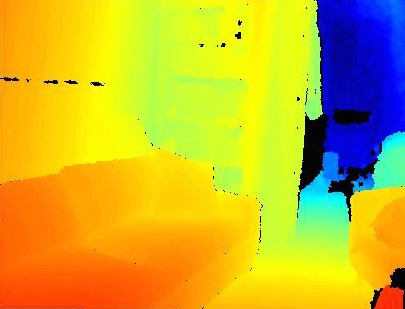
\includegraphics[height=2.1cm]{ogm_ex3.jpeg}\hspace*{0.1cm}
\hspace*{0.5cm}
    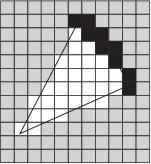
\includegraphics[height=2.1cm]{ogm_ex1.jpg}\hspace*{0.1cm}
\hspace*{0.5cm}
    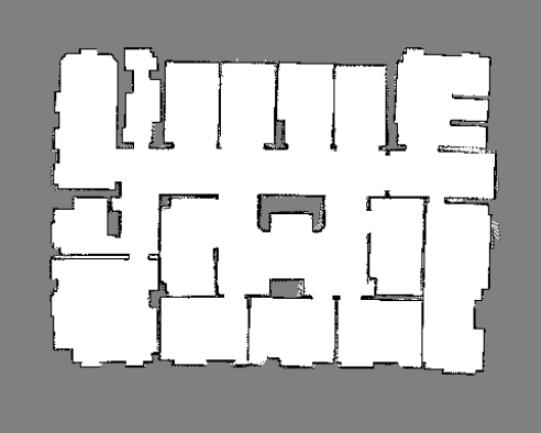
\includegraphics[height=2.1cm]{ogm_ex2.png}\hspace*{0.1cm}
}
\end{figure}}

\end{frame}






\begin{frame}
\frametitle{Problem Definition}
%\framesubtitle{Problem Definition}

\begin{itemize}
	\item The Map and the Robot
	\begin{itemize}
	\item Map $m$ is composed of $n_m$ grid cells with known location and size
	\item The $i$-th grid cell $\mathbf{m}_i$ is a \emph{static binary} random variable, independent of other grid cells: $P(m)=P(\mathbf{m}_1,\mathbf{m}_2,\ldots,\mathbf{m}_{n_m})=\prod_{i=1}^{n_m}P(\mathbf{m}_i)$
	\item \emph{Pose} $X_t$ is known, containing robot \emph{position} and \emph{attitude}
	\end{itemize}
\vspace*{0.0cm}\pause
\end{itemize}
\begin{minipage}[t]{7.0cm}
\begin{itemize}
	\item Depth Measurements
	\begin{itemize}
	\item Each measurement origin and direction is known \emph{deterministically}
	\item A measurement \emph{scan} $Z_t=\braces{z_{t,1},z_{t,2},\ldots,z_{t,n_z}}$ contains $n_z$ measurement \emph{rays} (depths)% at the $t$-th time step, and the history of measurement scans $Z_{1:t}$ is known
\item The \emph{forward sensor model} is known from the sensor properties
\end{itemize}
\end{itemize}
\end{minipage}
\begin{minipage}[t]{3.0cm}
%The \emph{forward sensor model} is the probability density distribution $p(z_{t,l}|m,X_{t})$  known from the sensor properties
\hspace*{0.25cm}
\begin{figure}[!htbp]
\vspace*{-0.25cm}
%\vspace*{0.25cm}
\centerline{
    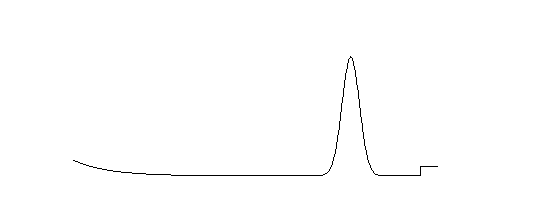
\includegraphics[width=3.5cm]{BeamModel.png}\hspace*{0.1cm}
    }
\vspace*{0.25cm}
\centerline{
    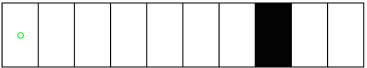
\includegraphics[width=2.5cm]{1D_True_Grid.png}\hspace*{0.1cm}
%    \hspace*{0.75cm}
    }
{Beam Model for Range Finders}
\end{figure}

\end{minipage}



\end{frame}

\begin{frame}
\frametitle{Problem Definition}

\begin{itemize}
	\item Bayesian Framework
	\begin{itemize}
	\item Markov Assumption: latest a priori cell occupancy probabilities capture the information from all prior observations
	\item Log-Odds Ratio: popular representation due to simple additive update structure and probability truncation avoidance, but requires the \emph{assumption}
	\begin{align*}
		P(Z_t|\mathbf{m}_i,X_{1:t},Z_{1:t-1})\approx P(Z_t|\mathbf{m}_i,X_t)
	\end{align*}
	\end{itemize}
\vspace*{0.0cm}\pause
	\item Inverse Sensor Model
	\begin{align*}
&P(\mathbf{m}_i|z_{t,l},X_{1:t},Z_{1:t-1})\nonumber
\\
&=\eta_{t,l}\sum_{m\in\mathcal{M}_i}p(z_{t,l}|m,X_{t})P(m|X_{1:t-1},Z_{1:t-1}).
\end{align*}
	\begin{itemize}
	\item Given $n$ grid cells: $\mathcal O(2^n)$ is \emph{computationally-intractable}, motivating a different solution
	\end{itemize}
\end{itemize}

\end{frame}

\begin{frame}
\frametitle{Inverse Sensor Model with Invariance}

\begin{itemize}
    \item Main idea: make use of occupancy grid mapping \emph{assumptions} and extract \emph{patterns} from probabilistic properties to find a \emph{computationally-efficient} solution
	\begin{itemize}
		\item Since the origin and direction of each measurement ray is known deterministically, the set of grid cells that the ray intersects is \emph{known through geometry}
		\item A depth reading follows the forward sensor model, which \emph{only depends} on the first occupied grid cell along the measurement ray
	\end{itemize}
\setcounter{subfigure}{0}
% uncomment
\vspace*{-0.03\textwidth}
\begin{figure}
  \centering
  \begin{subfigure}[t]{.45\linewidth}
    \centering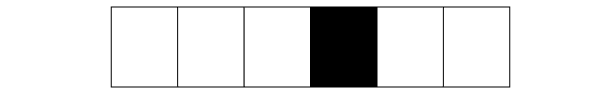
\includegraphics[width=\linewidth]{rkplus_1.png}
  \end{subfigure}
  \begin{subfigure}[t]{.45\linewidth}
    \centering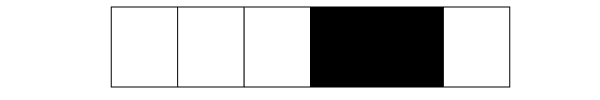
\includegraphics[width=\linewidth]{rkplus_2.png}
  \end{subfigure}
    \begin{subfigure}[t]{.45\linewidth}
    \centering
\includegraphics[width=\linewidth]{rkplus_3.png}
  \end{subfigure}
  \begin{subfigure}[t]{.45\linewidth}
    \centering
\includegraphics[width=\linewidth]{rkplus_4.png}
  \end{subfigure}
\end{figure}
	\item Avoids common approximated or learned solutions
\end{itemize}

\end{frame}




\begin{frame}
\frametitle{Bayesian Update}

\begin{itemize}
	\item Unnormalized Probability:
	\begin{align*}
\tilde P(\mathbf{r}_{k}|z,X_{1:t},Z_{1:t-1})
&=\mathbf{P}_k^-
\bigg[\sum_{i=1}^{k-1}\bigg\{\prod_{j=0}^{i-1}\bar{\mathbf{P}}_j^-\bigg\}p(z|\mathbf{r}_{i+},X_t)\mathbf{P}_k^-\bigg]\nonumber\\
&\qquad + \bigg\{\prod_{j=0}^{k-1}\bar{\mathbf{P}}_j^-\bigg\}p(z|\mathbf{r}_{k+},X_t)\mathbf{P}_k^-
\end{align*}
	\item Normalizer:
	\begin{align*}
\label{eqn:allEta}
\eta
&=
\bigg[\sum_{i=1}^{n_{r}+1}\bigg\{\prod_{j=0}^{i-1}\bar{\mathbf{P}}_j^-\bigg\} p(z|\mathbf{r}_{i+},X_t)\mathbf{P}_k^-\bigg]^{-1}
\end{align*}
	\item Solution: $P(\mathbf{r}_{k}|z,X_{1:t},Z_{1:t-1})=\eta\tilde P(\mathbf{r}_{k}|z,X_{1:t},Z_{1:t-1})$
	\item \emph{Linear Complexity}: $\mathcal{O}(n)$ for \emph{all} $n$ cells in FOV compared with $\mathcal O(n\times2^n)$ without using invariance
\end{itemize}
\end{frame}


\section*{}
\subsection*{Entropy-Based Autonomous Exploration}

\begin{frame}
\frametitle{Autonomous Exploration}

\begin{itemize}
	\item Goal: determine robotic actions that maximize map information
	\item Approach: predict future map uncertainty and travel distance to select an optimal pose
\end{itemize}

\end{frame}




\begin{frame}
\frametitle{Existing Exploration Approaches}

\begin{itemize}
	\item Frontier-Based Exploration
	\begin{itemize}
		\item A robot identifies boundaries of free and uncertain cells
		\item The robot moves toward these frontiers, thereby pushing back the boundaries
		\item Heuristic, suboptimal
	\end{itemize}
	\vspace*{0.0cm}\pause
	\item Entropy-Based Approaches
	\begin{itemize}
		\item Probabilities from the occupancy grid map are approximate
		\item Usage of ``hallucination measurements'': assume that $\text{E}[H(P(\mathbf{m}_i|z))]\approx H(P(\mathbf{m}_i|\text{E}[z]))$
	\end{itemize}
	\vspace*{0.0cm}\pause
	\item Proposed Approach
	\begin{itemize}
		\item Use occupancy grid map probabilities
		\item Solve $\text{E}[H(P)]$ and select future poses to maximize map information
	\end{itemize}
\end{itemize}
\end{frame}

\begin{frame}
\frametitle{Entropy Definition}
\begin{itemize}
        	\item Uncertainty-Based Exploration
	\begin{itemize}
		\item Main idea: choose robot motions that minimize the uncertainty of the occupancy grid map
		\item Equivalently maximize map information gain
	\end{itemize}
\end{itemize}
\begin{minipage}[t]{7.0cm}
\begin{itemize}
	\item Entropy
	\begin{itemize}		
		\item \emph{Shannon's entropy} serves as an uncertainty measure
		\begin{align*}
			H(P)=-P\log P-\bar{P}\log \bar{P}%-(1-P)\log(1-P)
		\end{align*}
		with cell occupancy probability $P$ and complement $\bar{P}=1-P$
		\item Entropy $H$ is maximized when $P=0.5$ and minimized as $P\rightarrow0$ or $P\rightarrow1$
	\end{itemize}
\end{itemize}
\end{minipage}
\begin{minipage}[t]{3.0cm}
\vspace*{0.5cm}
\begin{figure}[!htbp]
	\centerline{
		\hspace*{1.25cm}
   		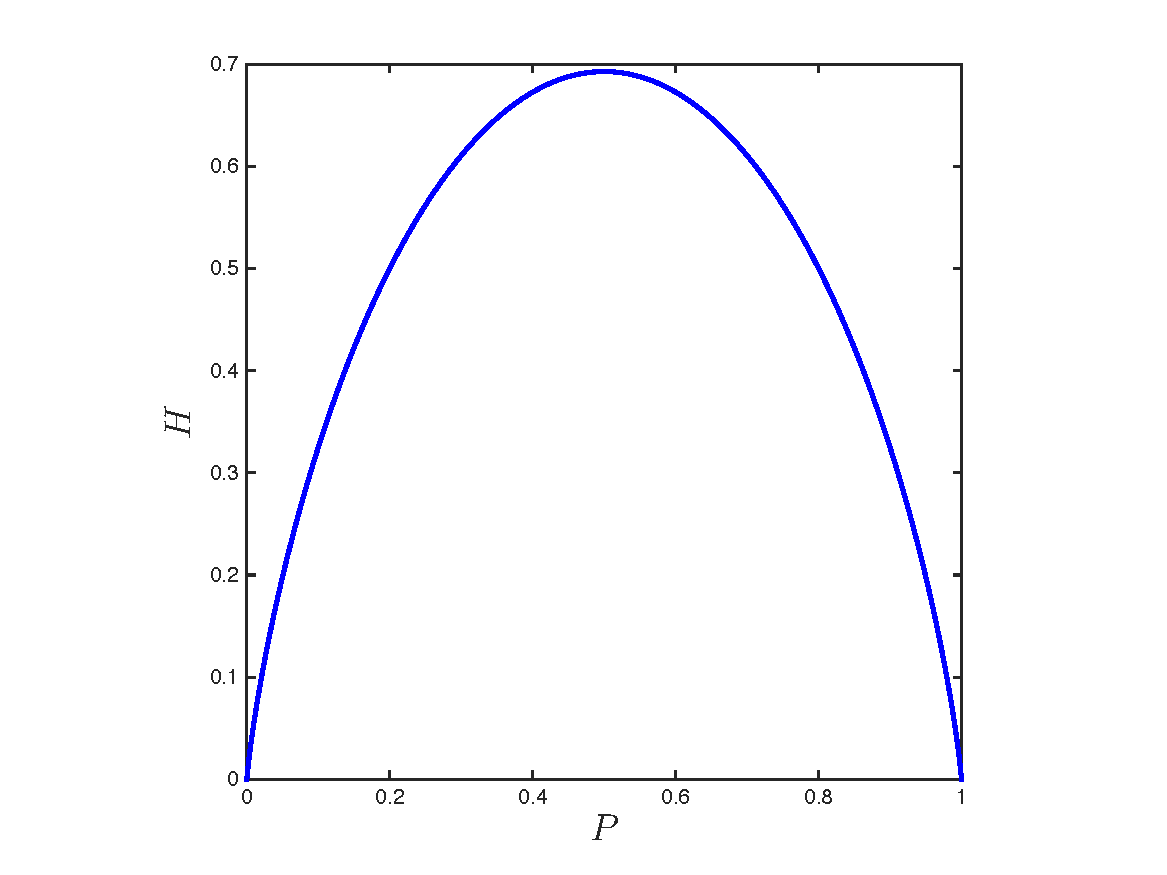
\includegraphics[width=5.0cm]{H_Plotted_square.pdf}%\hspace*{0.1cm}
	}
\end{figure}
\end{minipage}

\end{frame}



\begin{frame}
\frametitle{Expected Information Gain}

\begin{itemize}
	\item Main Idea: determine the benefit of future poses based on how their measurements are expected to improve the map
	\vspace*{0.0cm}\pause
	\item Goal: decrease total map entropy:
	\begin{align*}
		H(P(m))&=\sum_{i=1}^{n_m}H(P(\mathbf{m}_i))
	\end{align*}
	\vspace*{0.0cm}\pause
	\item Measurement Ray Expected Information Gain:
	\begin{align*}
		\text{E}[H(P(m|x_c,z_{c}))]&=\sum_{k=1}^{n_{r}+1}\bigg\{H(P(m|x_c,z_{c,k}))P(z_{c,k}|x_c)\bigg\}
		\\
		P(z_{c,k}|x_c)&=\frac{p(z_{c,k}|x_c)}{\sum_{i=1}^{n_{r}+1}p(z_{c,i}|x_c)}=\frac{\eta_{c,k}^{-1}}{\sum_{i=1}^{n_{r}+1}\eta_{c,i}^{-1}}
		\\
		\mathcal I(x_c,z_{c})&=H(P(m))-\text{E}[H(P(m|x_c,z_{c}))]
	\end{align*}
\end{itemize}

\end{frame}

\begin{frame}
\frametitle{Pose Information Gain in 2D}

\begin{itemize}
	\item Main Idea: select the future pose that maximizes map information gain while accounting for travel distance
	\vspace*{0.0cm}\pause
	\item Attitude Selection: choose the attitude that covers the candidate measurement rays with largest objective function summation
\begin{figure}
\centerline{
	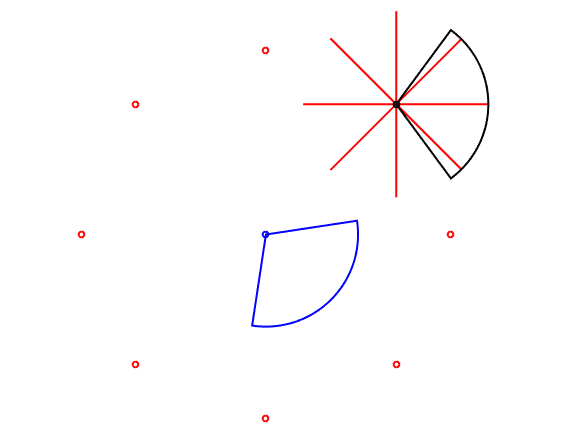
\includegraphics[height=0.35\linewidth]{ExampleOptimalPose.png}
%\begin{picture}(0,0)(0,0)
%\setlength{\unitlength}{0.1\linewidth}\scriptsize
%\put(4.4,2.1){\color{blue}$X_t$}
%\put(5.9,1.9){\color{red}$x_1$}
%\put(2.9,2.0){\color{red}$x_5$}
%\put(4.4,3.6){\color{red}$x_3$}
%\put(4.4,0.6){\color{red}$x_7$}
%\put(5.4,3.0){\color{red}$x_2$}
%\put(3.3,3.1){\color{red}$x_4$}
%\put(3.3,1.0){\color{red}$x_6$}
%\put(5.4,1.0){\color{red}$x_8$}
%\put(6.8,3.1){\color{red}$z_{2,1}$}
%\put(4.5,3.1){\color{red}$z_{2,5}$}
%\put(5.6,4.1){\color{red}$z_{2,3}$}
%\put(5.6,2.2){\color{red}$z_{2,7}$}
%\put(6.5,3.7){\color{red}$z_{2,2}$}
%\put(4.9,3.8){\color{red}$z_{2,4}$}
%\put(5.0,2.5){\color{red}$z_{2,6}$}
%\put(6.5,2.5){\color{red}$z_{2,8}$}
%\put(6.1,2.9){$X_c^*$}
%\end{picture}
}
\vspace*{-0.05\linewidth}
\end{figure}
	\item The attitude $R_c$ is selected for all candidates: the expected information gain becomes $\mathcal I(X_c)$ where $X_c=\braces{x_c,R_c}$
\end{itemize}

\end{frame}


\begin{frame}
\frametitle{Pose Information Gain in 3D}

\begin{itemize}
	\item Several sample pitch angles per horizontal direction
	\item Optimal attitude assuming level flight, i.e., zero roll/pitch
	\item Consideration of grid cells above and below the vehicle
\end{itemize}
\begin{figure}[!t]
	\centering
	\begin{subfigure}[t]{0.3\columnwidth}
           	\centering
          	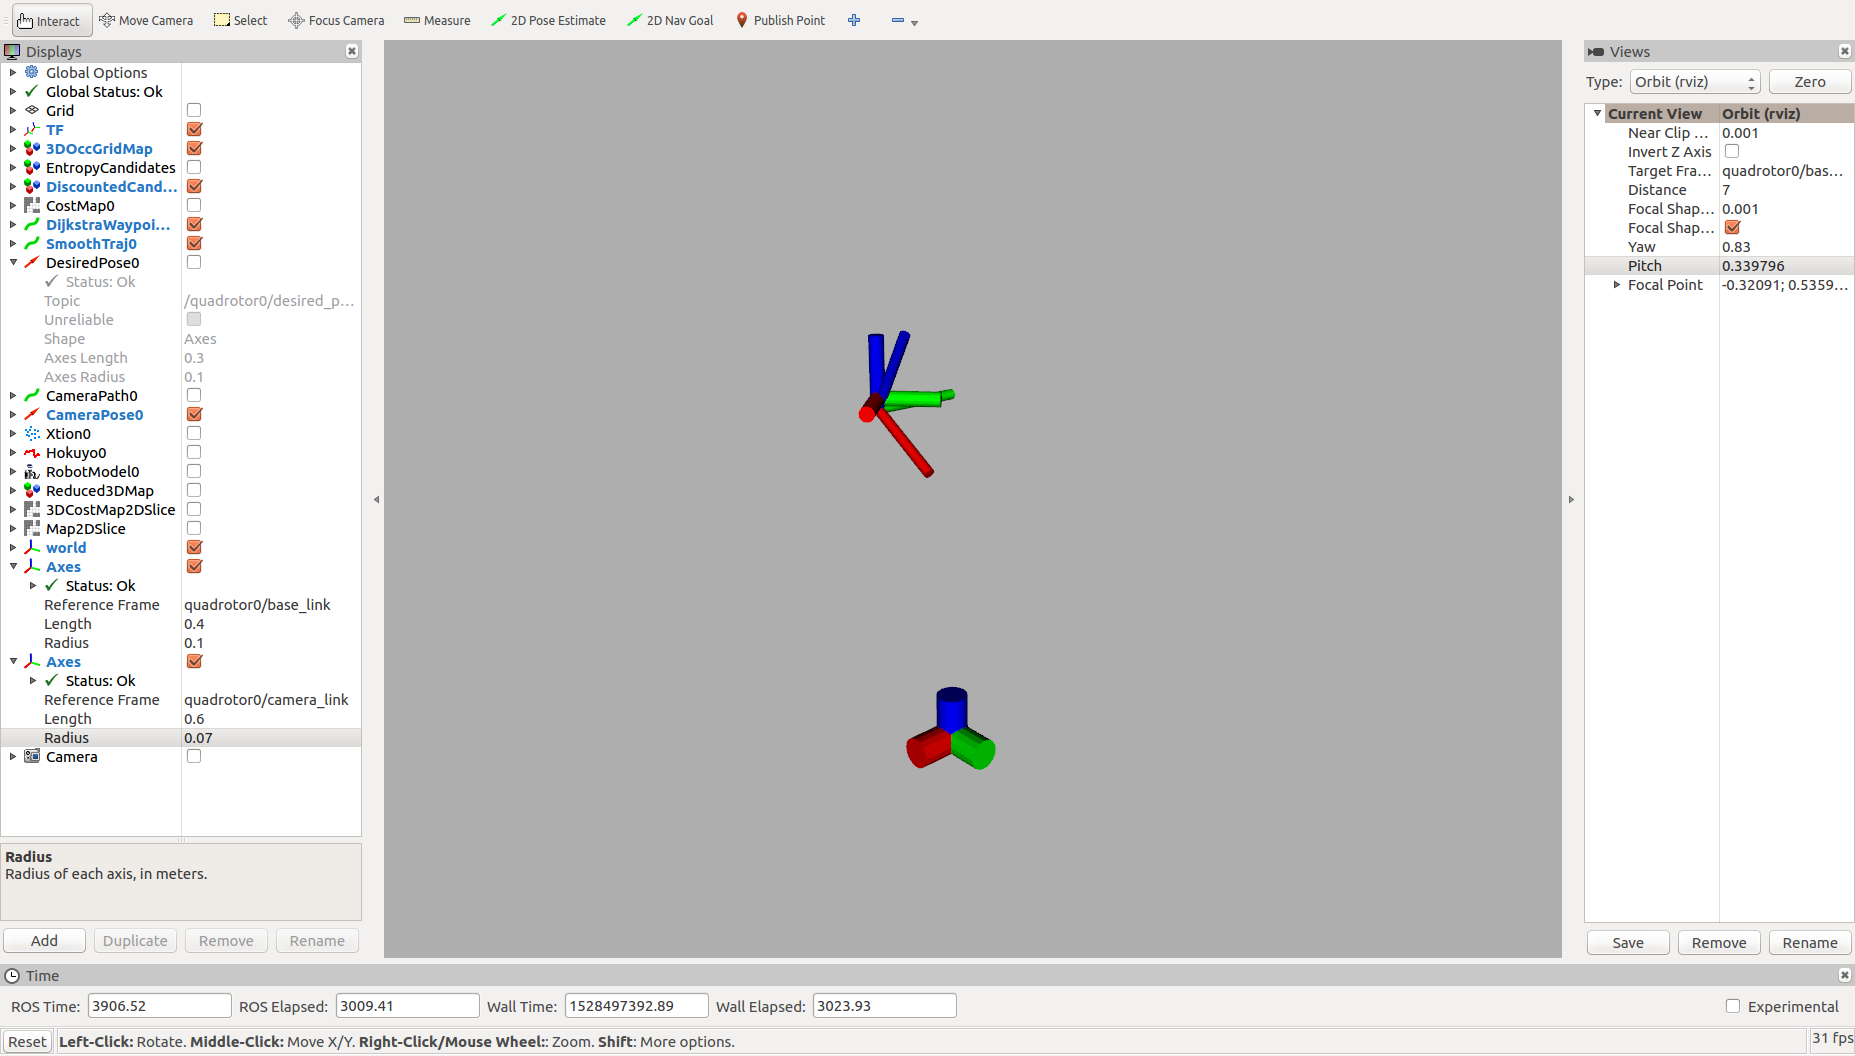
\includegraphics[trim = {21cm 5cm 20cm 5cm}, clip, height=1.0\textwidth]{mars_general.png}
        		\caption{General View}
    	\end{subfigure}
    	\begin{subfigure}[t]{0.3\columnwidth}
           	\centering
          	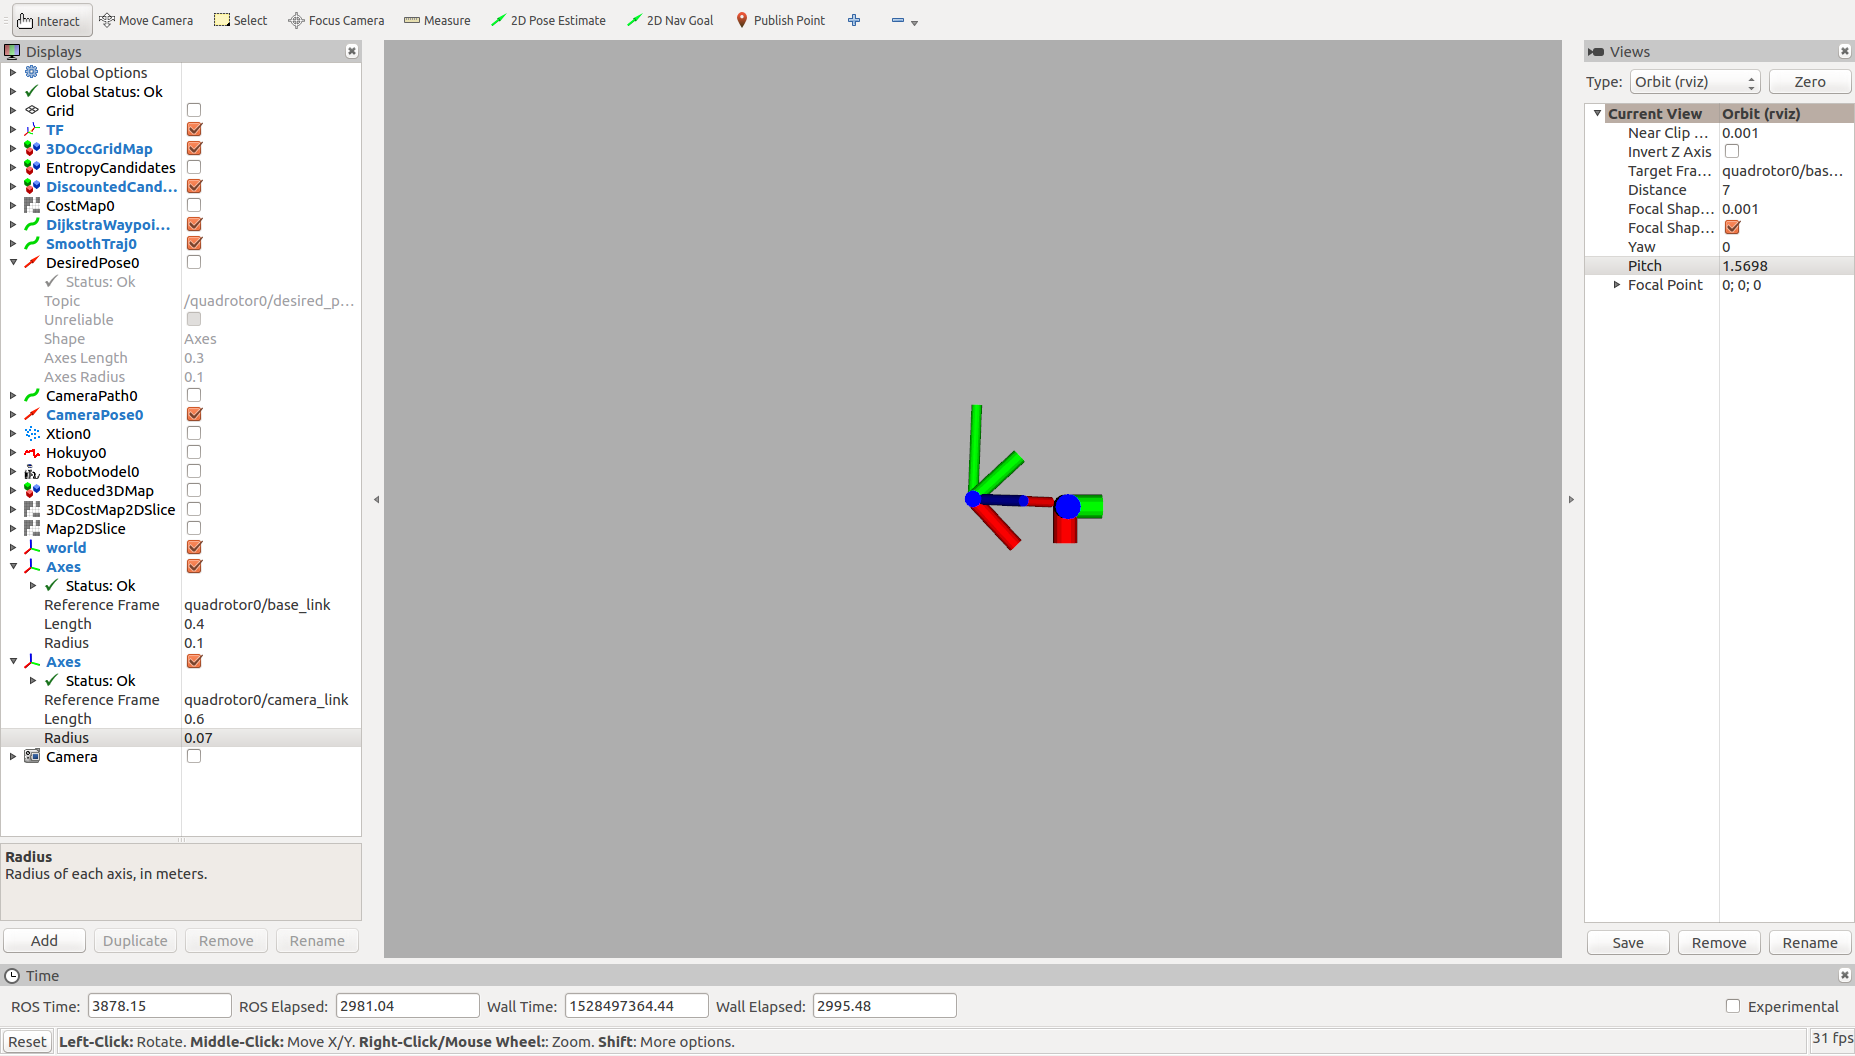
\includegraphics[trim = {25cm 6cm 16cm 4cm}, clip, height=1.0\textwidth]{mars_psi.png}
        		\caption{$\psi$ Rotation}
    	\end{subfigure}
	\begin{subfigure}[t]{0.3\columnwidth}
           	\centering
          	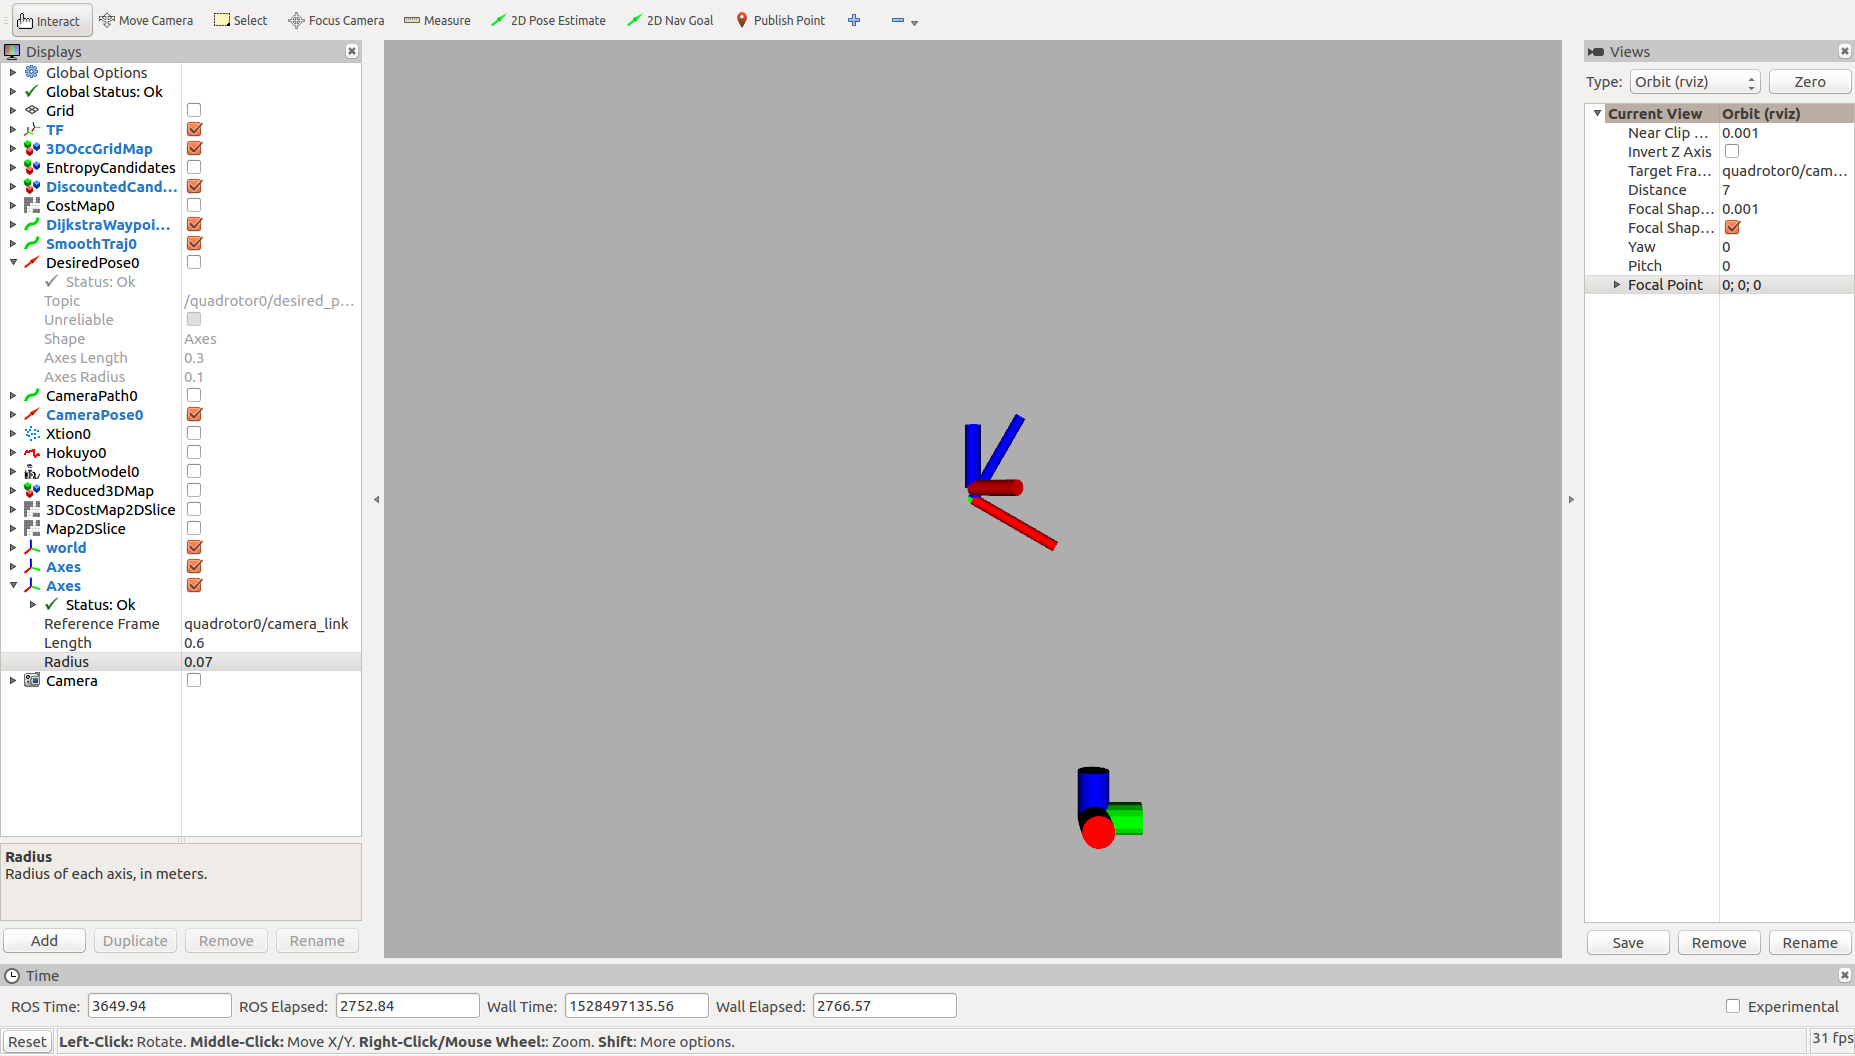
\includegraphics[trim = {23cm 4cm 17cm 6cm}, clip, height=1.0\textwidth]{mars_theta.png}
        		\caption{$\theta$ Rotation}
    	\end{subfigure}
%\includegraphics[width=2.5in]{myfigure}
% where an .eps filename suffix will be assumed under latex, 
% and a .pdf suffix will be assumed for pdflatex; or what has been declared
% via \DeclareGraphicsExtensions.
\label{fig:transforms}
\end{figure}
\end{frame}


\begin{frame}
\frametitle{Pose Selection}

\begin{itemize}
	\item Travel Distance: generate a cost map from the occupancy grid to obtain distances to each candidate pose $d(x_c)$
	\vspace*{0.0cm}\pause
	\item Bump Function: use a bump function \begin{align*}f(d)=\exp\braces{-\frac{d^2}{2\sigma^2}}+\gamma, \quad \sigma>0, \quad \gamma>0\end{align*} to incentivize the robot to explore more locally until nearby spaces are well-known
	\begin{figure}
	\vspace*{-0.015\linewidth}
\centering
	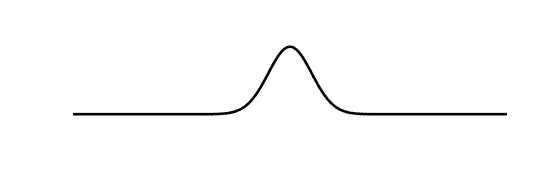
\includegraphics[width=0.8\linewidth]{GaussianBumpFunFlat.png}
		\vspace*{-0.015\linewidth}
\end{figure}
	% C++: exp(-0.5*distAway*distAway/sigSqrd)+minFunVal GaussianBumpFunFlat.png
	\vspace*{0.0cm}\pause
	\item Select the pose that maximizes the product \begin{align*}X^*=\argmax_{X_c}{\mathcal I(X_c)f(d(x_c))}\end{align*}
\end{itemize}

\end{frame}


\begin{frame}
\frametitle{Collision-Free Path}

\begin{itemize}
	\item Using the cost map from before, \emph{Dijkstra's algorithm} is completed by finding the waypoints from the desired candidate back to the current location
	\vspace*{0.0cm}\pause
	\item These waypoints serve as input to a \emph{constrained polynomial least squares trajectory}
	\begin{itemize}
		\item Each trajectory is solved independently as a function of time, i.e. $x(t)$, $y(t)$
		\item Starting and terminal locations are fixed
		\item Segments patched together have the same position and velocity at the connection
	\end{itemize}
	\vspace*{0.0cm}\pause
	\item A \emph{geometric controller} tracks the trajectory without \emph{singularities} or \emph{ambiguities}
	\vspace*{0.0cm}\pause
	\item The mapping, exploration, and control run in \emph{real-time}
\end{itemize}

\end{frame}

\begin{frame}
\frametitle{Optimal Pose Selection in 3D}

\begin{itemize}
	\item Apply Dijkstra's algorithm about 3D graph of occupancy grid
	\item Locations and associated distance costs for reachable positions in 3D
\end{itemize}
\begin{figure}
	\centering
	\begin{subfigure}[t]{0.45\columnwidth}
           	\centering
          	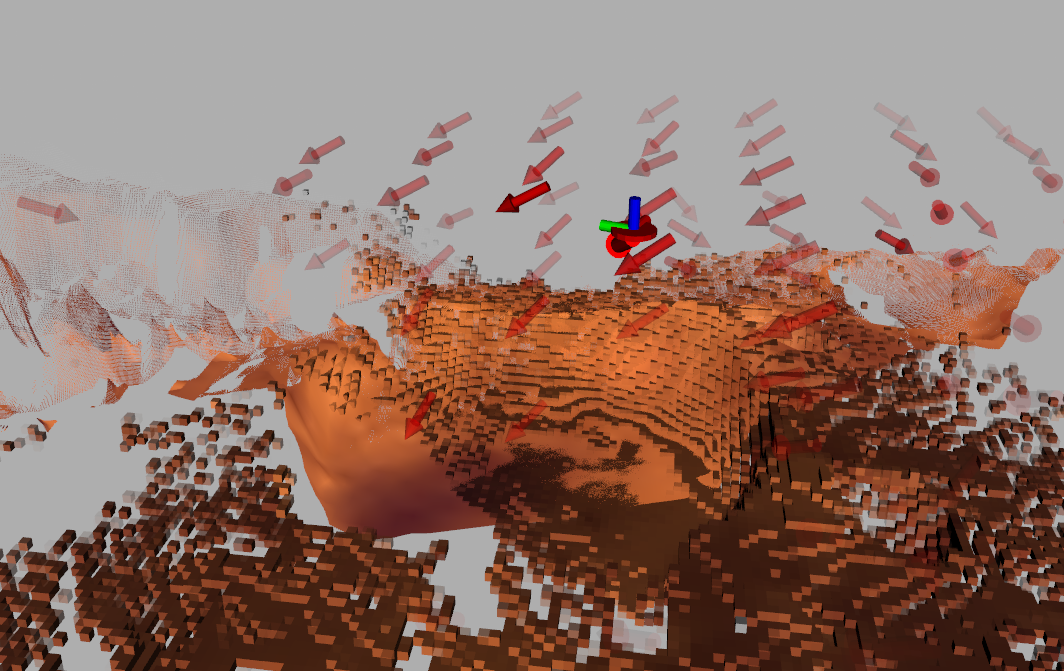
\includegraphics[height=0.5\textwidth]{mars_closeup.png}
        		\caption{Mars Simulation Poses}
    	\end{subfigure}
	\begin{subfigure}[t]{0.45\columnwidth}
           	\centering
          	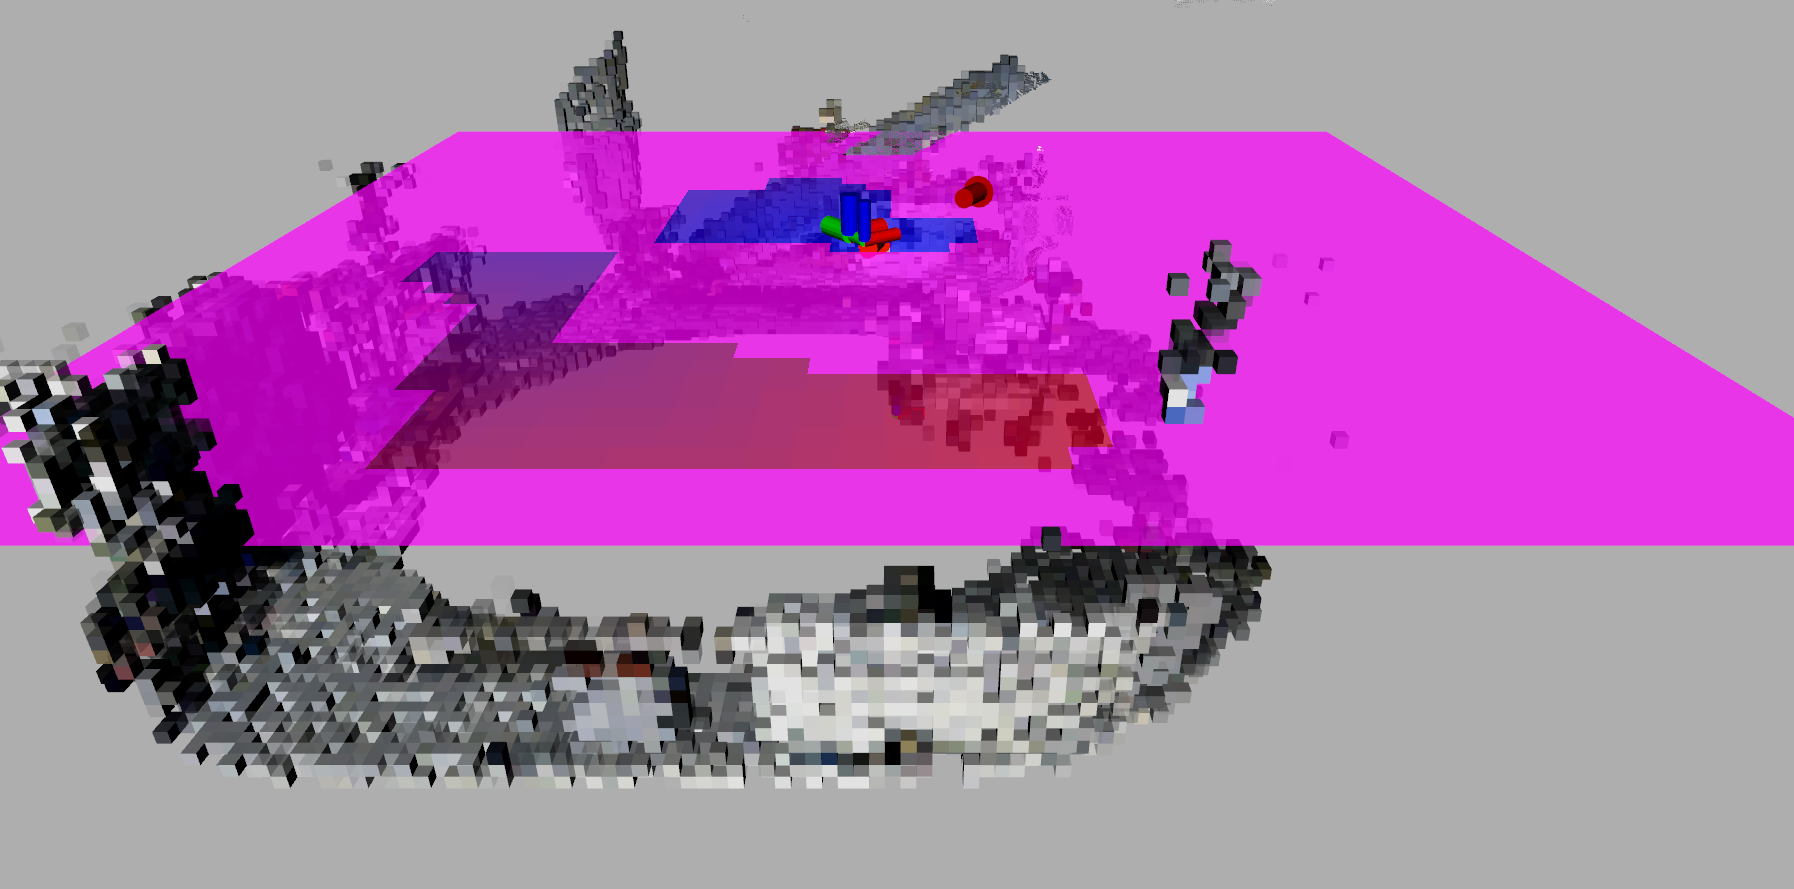
\includegraphics[height=0.5\textwidth]{disconnected_costmap.png}
        		\caption{3D Dijkstra's Search}
    	\end{subfigure}
\label{fig:marsZoomedIn}
\end{figure}
\end{frame}

\begin{frame}
	\frametitle{3D Mars Exploration Conclusions}
	\begin{itemize}
		\item Expected information gain of several poses in 3D space capturing complex obstacles
		\item Distance cost accounts for collision-avoidance
		\item Mapping and exploration are computationally-efficient for real-time implementation
	\end{itemize}
		\begin{figure}
		\centerline{
			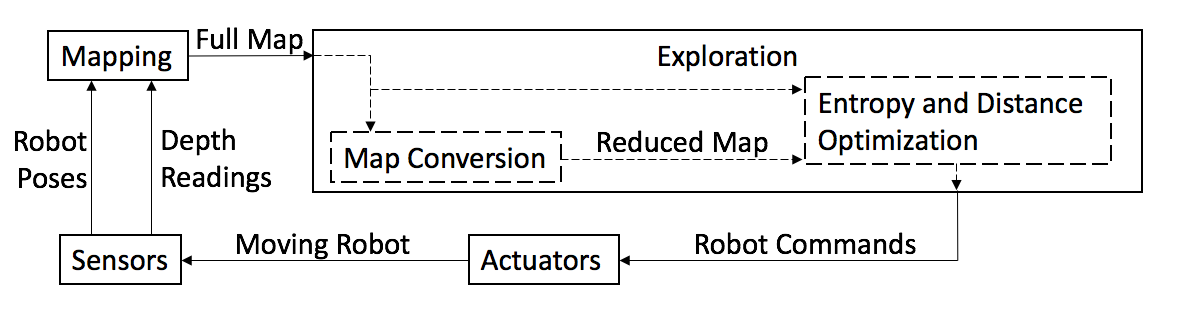
\includegraphics[width=0.8\columnwidth]{node_diagram_3D_mars.png}
		}
		\label{fig:NodesDiagram}
	\end{figure}
\end{frame}


\section*{}
\subsection*{Numerical Simulation \& Experiment}

\begin{frame}
	\frametitle{3D Autonomous Exploration Mars}
	\begin{itemize}
		\item A color image of Mars is draped over its height map using the Gazebo simulator
		\item Mapping and autonomous exploration are run in real-time using ROS nodes
		\item 3D depth measurements are simulated with Gaussian noise
		\item The robot is free to move within free space inside a fixed 3D volume
	\end{itemize}
	\begin{figure}[!t]
		\centering
		\begin{subfigure}[t]{0.3\columnwidth}
           		\centering
          		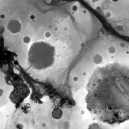
\includegraphics[height=0.9\textwidth]{mars_heightmap.png}
        			\caption{Height Map}
    		\end{subfigure}
    		\begin{subfigure}[t]{0.3\columnwidth}
			\centering
			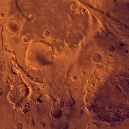
\includegraphics[height=0.9\textwidth]{mars_colormap.png}
      	  		\caption{Color Map}
   	 	\end{subfigure}
  	  	\begin{subfigure}[t]{0.3\columnwidth}
			\centering{
          		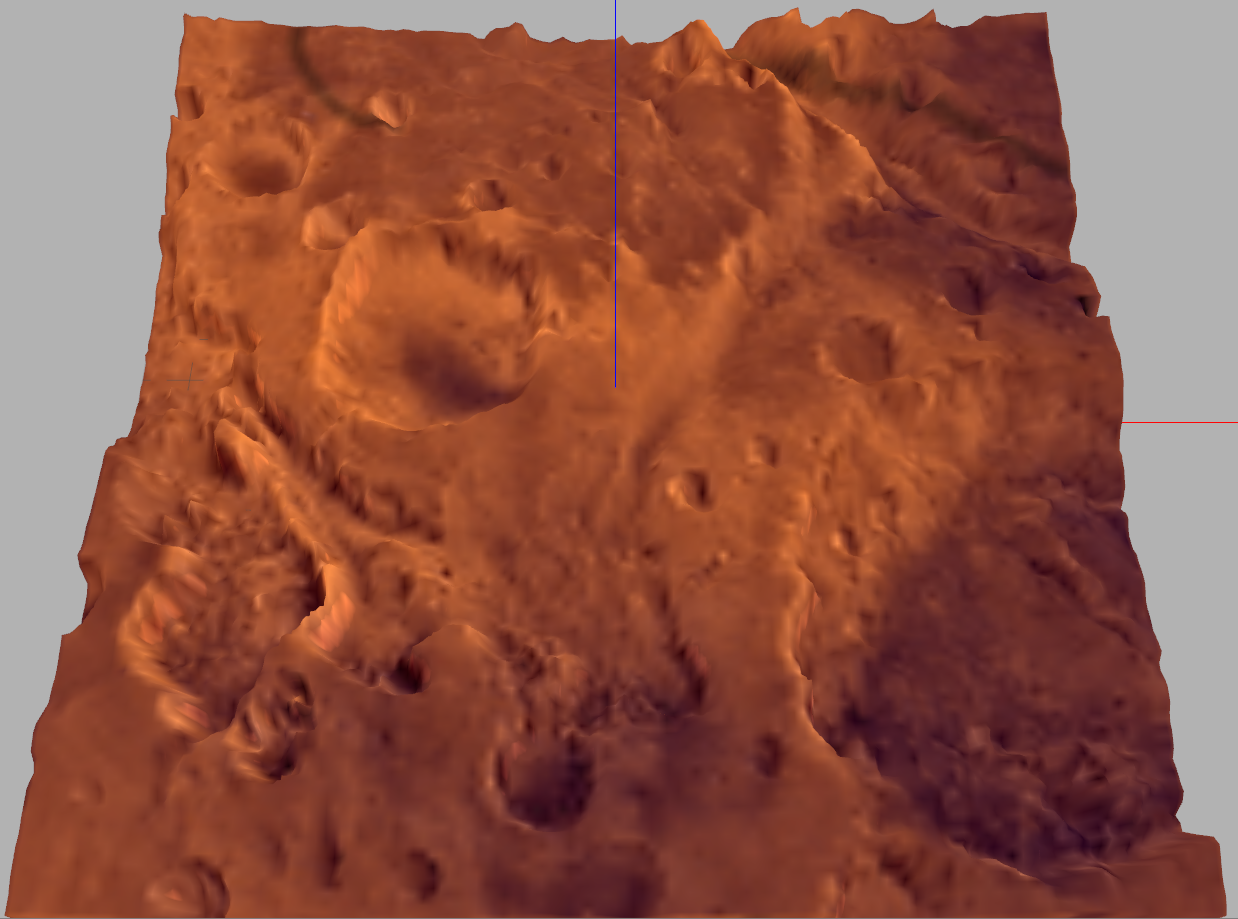
\includegraphics[height=0.9\textwidth]{mars_gazebo_full_lighting.png}}
        			\caption{Gazebo}
    		\end{subfigure}
	\label{fig:MarsGazebo}
	\end{figure}
\end{frame}

\begin{frame}
	\frametitle{Mars Video}
	\centering{
		\includemedia[
  		width=\textwidth,
  		height=0.8\textwidth,
  		activate=pageopen,
  		addresource=Topological Mars Mapping and Autonomous Exploration in 3D.mp4,
  		flashvars={source=Topological Mars Mapping and Autonomous Exploration in 3D.mp4}
		]{}{VPlayer.swf}
		}
\end{frame}


\begin{frame}
\frametitle{Experiment: Aerial Vehicle in a Complex 3D Environment}
\begin{itemize}
        	\item Full 3D mapping and exploration
	\item Objects are not vertically-uniform
	\item Environment Size: $9.0$ m $\times$ $8.5$ m $\times$ $2.25$ m
\end{itemize}


\begin{figure}
  \centering
  \begin{subfigure}[t]{.4\linewidth}
    \centering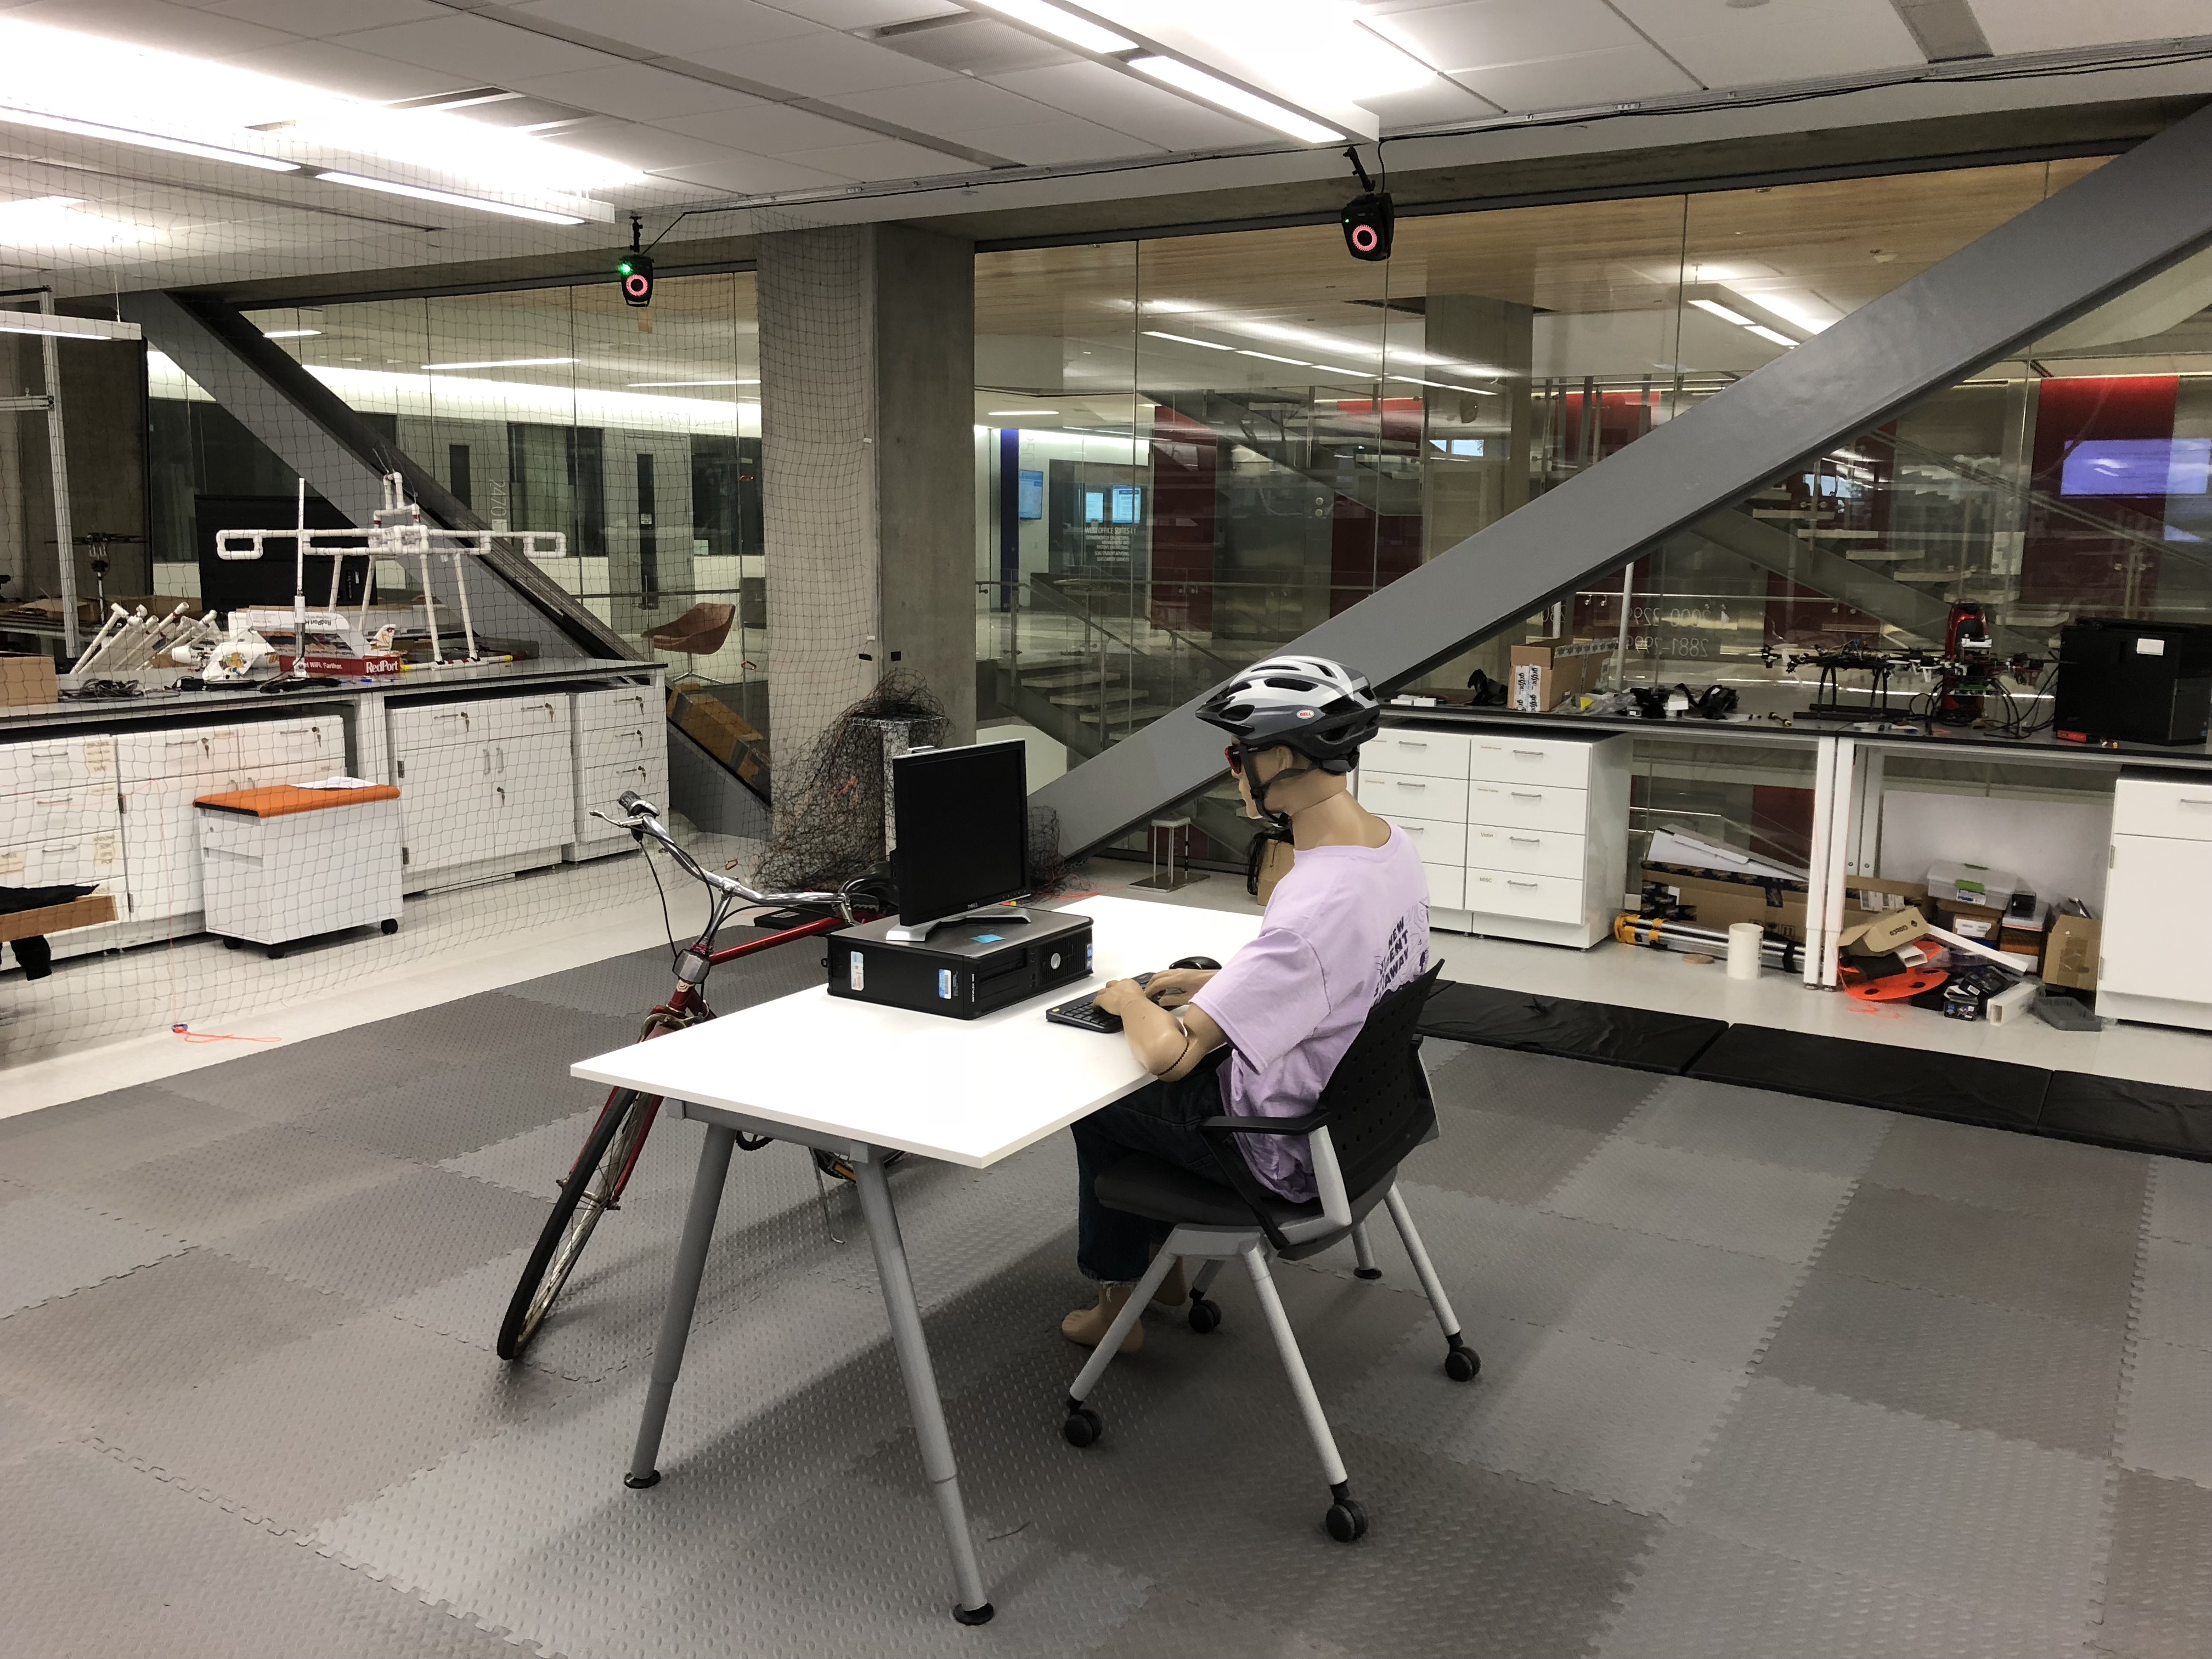
\includegraphics[height=.7\linewidth]{explore3D_space_NW.JPG}
    \caption*{Northwest View}
  \end{subfigure}
  \begin{subfigure}[t]{.4\linewidth}
    \centering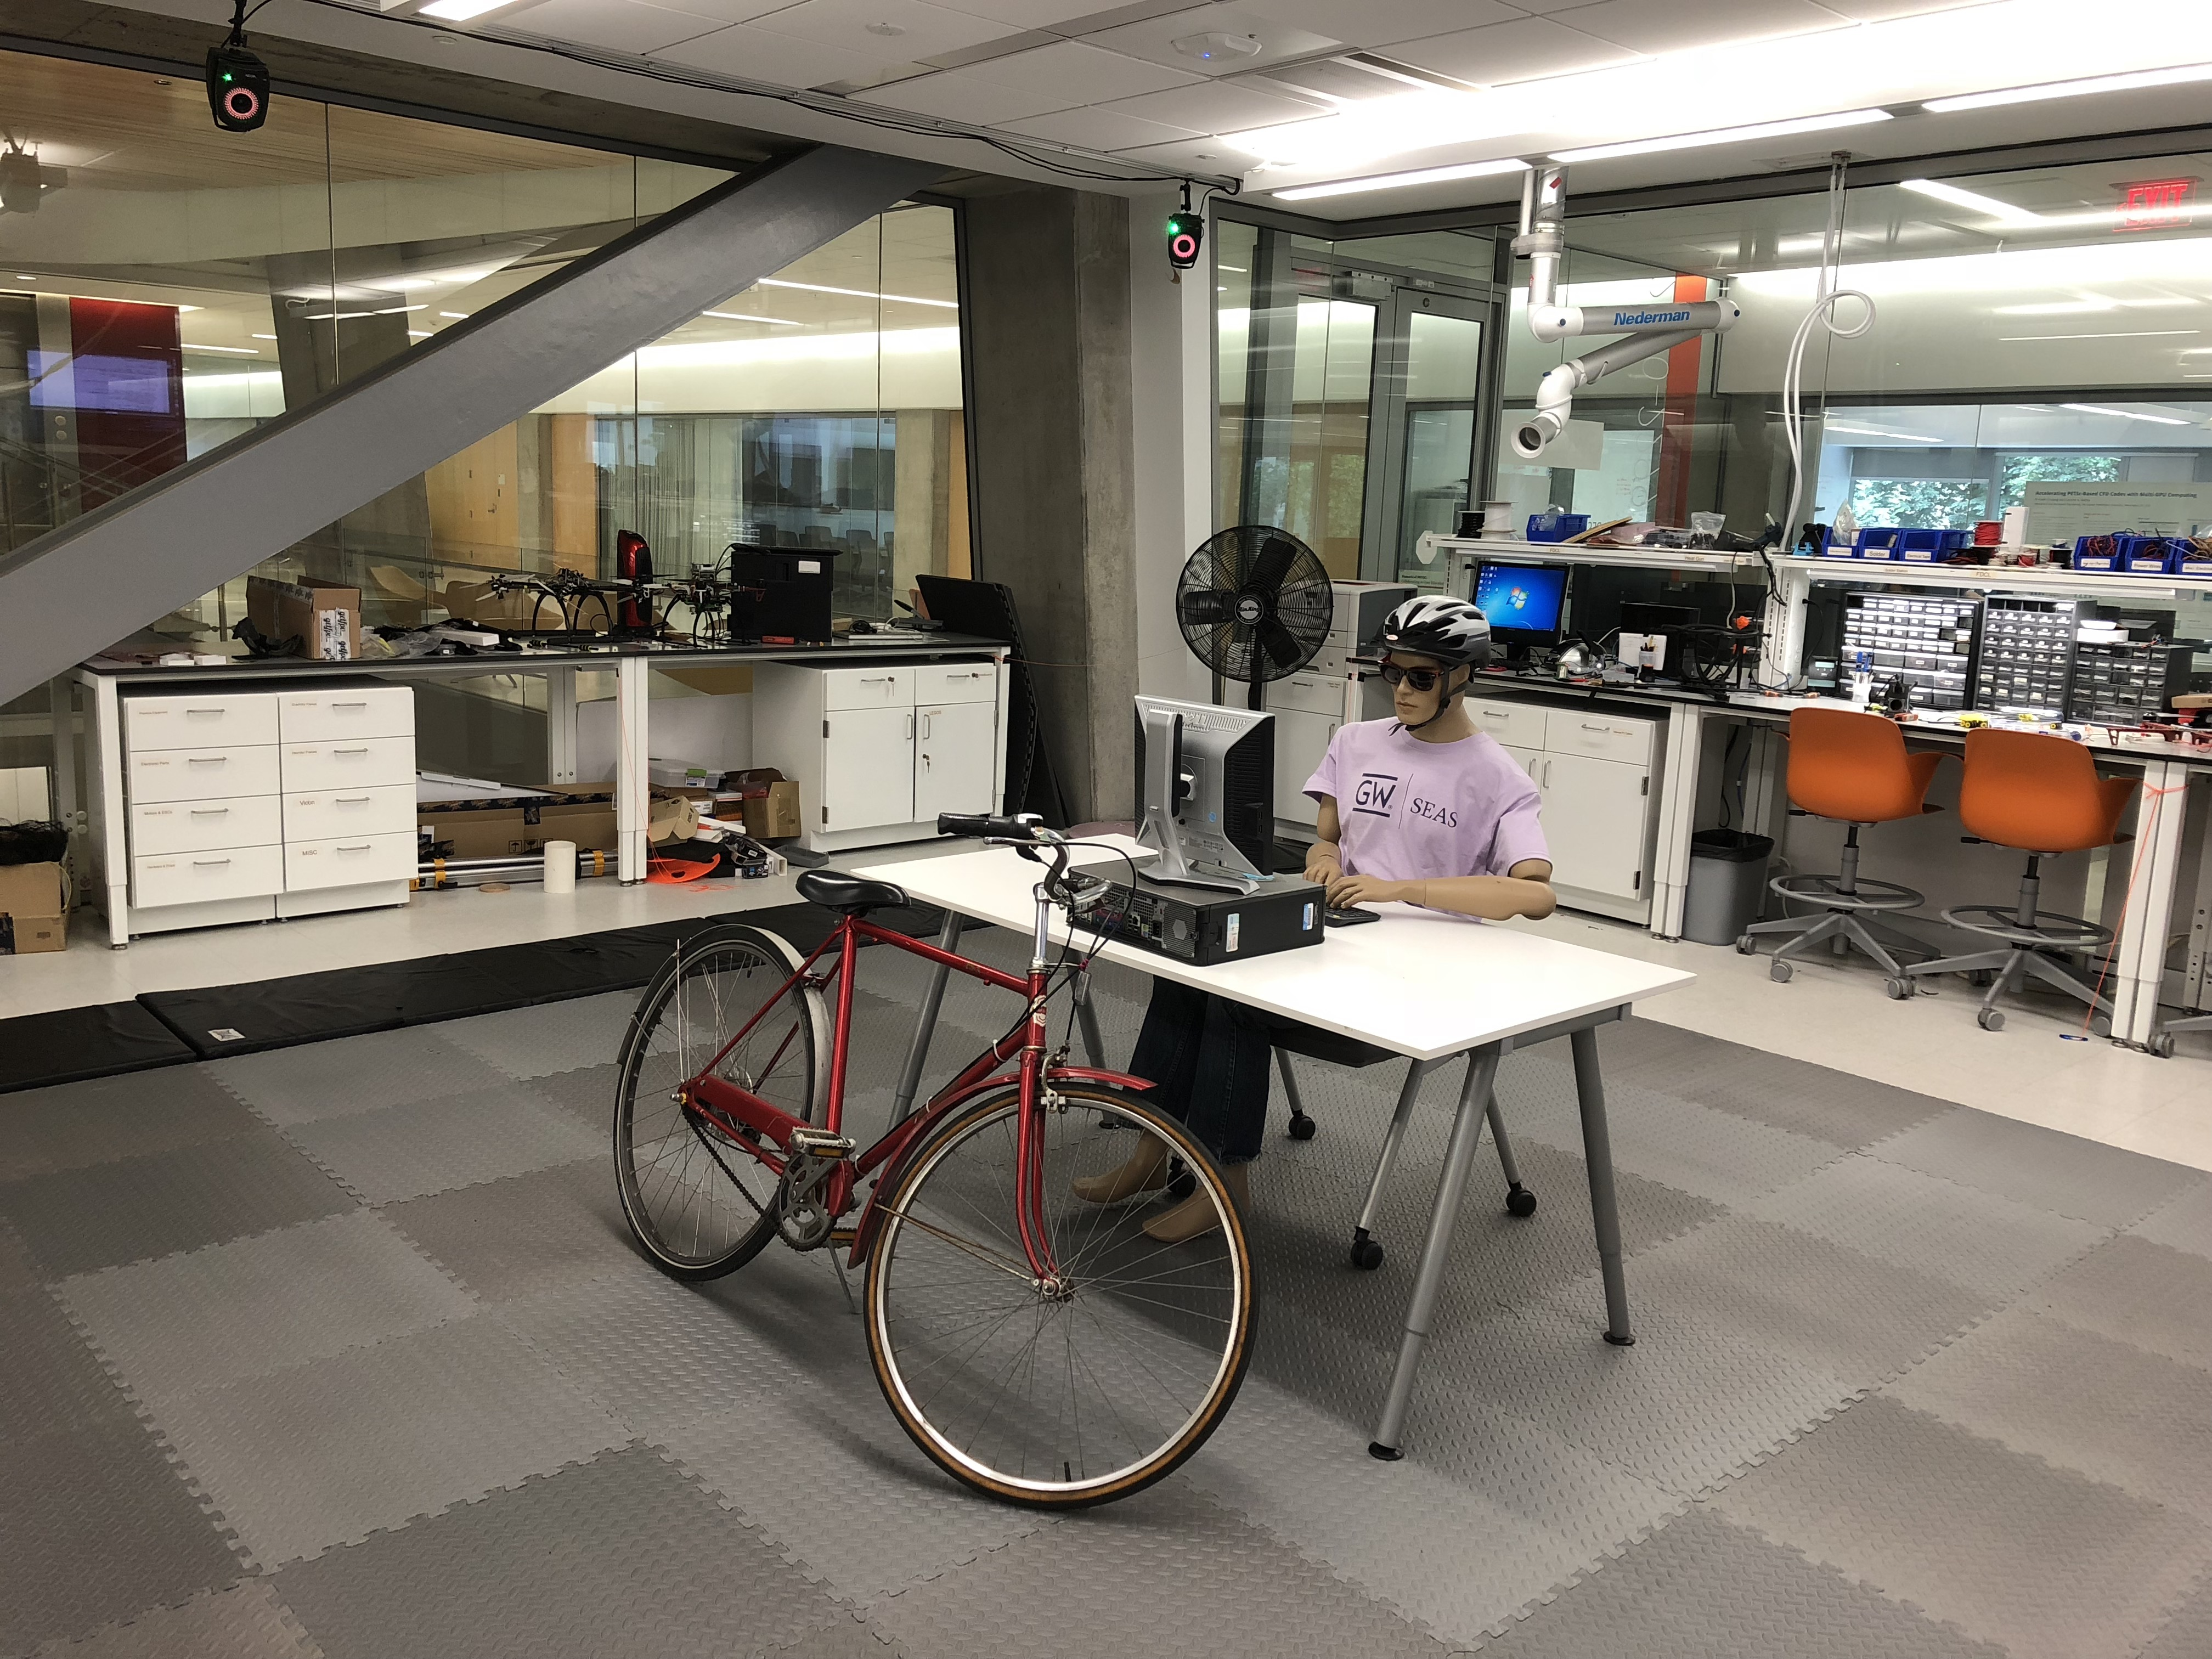
\includegraphics[height=.7\linewidth]{explore3D_space_NE.JPG}
    \caption*{Northeast View}
  \end{subfigure}
\end{figure}
\end{frame}


\begin{frame}
\frametitle{Full 3D Aerial Experiment Video}


	\centering{
		\includemedia[
  		width=\textwidth,
  		height=0.8\textwidth,
  		activate=pageopen,
  		addresource=explore3D_SEH.mp4,
  		flashvars={source=explore3D_SEH.mp4}
		]{}{VPlayer.swf}
		}


\end{frame}

\begin{frame}
\frametitle{Experiment Summary}
\begin{itemize}
        	\item Environments in complex 3D are modeled with occupancy grids in simulation and experimentation
	\item Predicted entropy of certain and uncertain spaces provide a policy for 3D autonomous exploration
	\item Dijkstra's search provides a collision-free path and estimated travel costs that account for obstacles
	\item All algorithms are run in real-time without expensive post-processing 
\end{itemize}
\end{frame}

\section*{}
\subsection*{Conclusions}

\begin{frame}
\frametitle{Conclusions}
\begin{itemize}
        	\item Proposed an occupancy grid mapping technique that uses the \emph{exact probabilistic solution}
	\item Computational cost is reduced \emph{substantially} for \emph{real-time implementation} using probabilisitic properties and exploiting mathematical patterns
	\item Exact mapping concepts are extended to map uncertainty to accomplish \emph{autonomous exploration}
	\item Multiple vehicles can explore and patrol an uncertain environment using a \emph{bidding}-based approach
	\item These are demonstrated with numerous simulations and experiments
\end{itemize}
\end{frame}

\end{document}

